% -*- root: Document.tex -*-

\chapter{\SS{} Architecture}
\label{chap:arch}

The architecture of \SS{} comprises a combination of two different types of base components: \textsf{worker} and \textsf{router}.
A \textsf{worker} component continuously listens for incoming data by means of non-blocking I/O.
As soon as data flows in, an application-dependent business logic is applied.
A typical use-case is the deployment of a classic filter/map/reduce pattern from the functional programming paradigm~\cite{bird_introduction_1988}.
In such a case, worker nodes execute only one function, namely \texttt{map}, \texttt{filter}, or \texttt{reduce}.
A \textsf{router} component acts as a message broker between workers in the pipeline and transfers data between them according to a given \emph{dispatching policy}.
Figure~\ref{fig:architecture_pipeline} depicts a possible implementation of this dataflow pattern using the \SS{} middleware.

\begin{figure}[t]
  \centering
  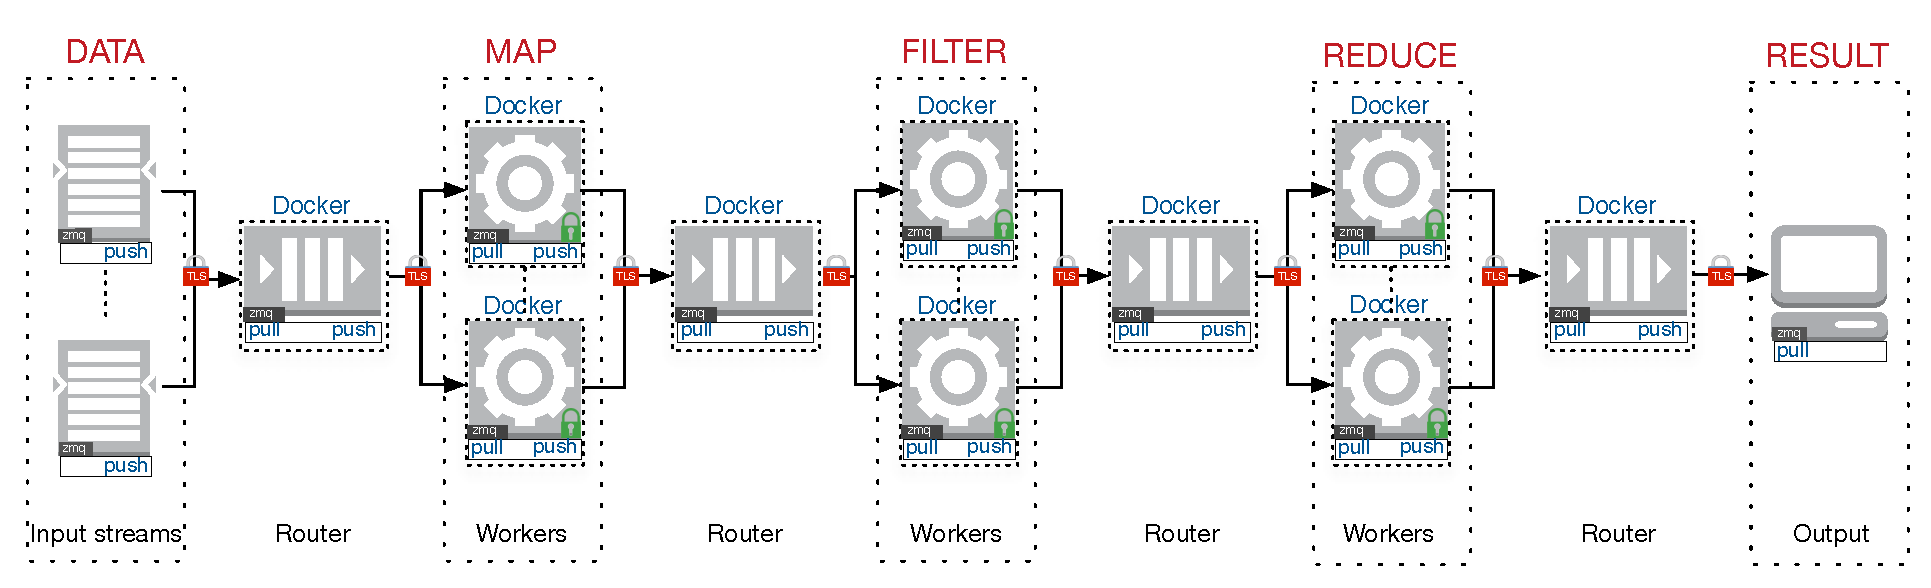
\includegraphics[width=\linewidth]{Figures/architecture_pipeline}
  \caption{Example of \SS{} pipeline architecture.}
  \label{fig:architecture_pipeline}
\end{figure}


\SS{} is designed to support the processing of sensitive data inside SGX enclaves.
As explained in the previous section, the \emph{enclave page cache} (EPC) is currently limited to $128\,\mathit{MB}$.
To overcome this limitation, we settled on a lightweight yet efficient embeddable runtime, based on the \textsc{Lua} virtual machine (\luavm)~\cite{ierusalimschy_luaextensible_1996} and the corresponding multi-paradigm scripting language~\cite{lualang}.
The \textsc{Lua} runtime requires only few kilobytes of memory, it is designed to be embeddable, and as such it represents an ideal candidate to execute in the limited space allowed by the EPC.
Moreover, the application-specific functions can be quickly prototyped in \textsc{Lua}, and even complex algorithms can be implemented with an almost 1:1 mapping from pseudo-code~\cite{leonini2009splay}.
We provide further implementation details of the embedding of the \luavm inside an SGX enclave in Section~\ref{chap:proto}.

Each component is wrapped inside a lightweight Linux container (in our case, the \emph{de~facto} industrial standard Docker~\cite{docker}).
Each container embeds all the required dependencies, while guaranteeing the correctness of their configuration, within an isolated and reproducible execution environment.
By doing so, a \SS{} processing pipeline can be easily deployed without changing the source code on different public or private infrastructures.
For instance, this will allow developers to deploy \SS{} to Amazon EC2 container service~\cite{awsec2container}, where SkyLake-enabled instances will soon be made available~\cite{amazonskylake}, or similarly to Google compute engine~\cite{gceskylake}.
The deployment of the containers can be transparently executed on a single machine or a cluster, using a Docker network and the Docker Swarm scheduler~\cite{docker:swarm_2016}.

The communication between workers and routers leverages \zmq{}, a high-performance asynchronous messaging library~\cite{zero_mq}.
Each router component hosts inbound and outbound queues.
In particular, the routers use the \zmq's pipeline pattern~\cite{zero_mq:pipeline} with the \textsc{Push}-\textsc{Pull} socket types.

The inbound queue is a \textsc{Pull} socket.
The messages are streamed from a set of anonymous\footnote{\emph{Anonymous} refers to a peer without any identity: the server socket ignores which worker sent the message.} \textsc{Push} peers (\textit{e.g.}, the upstream workers in the pipeline).
The inbound queue uses a fair-queuing scheduling to deliver the message to the upper layer.
Conversely, the outbound queue is a \textsc{Push} socket, sending messages using a round-robin algorithm to a set of anonymous \textsc{Pull} peers---\textit{e.g.}, the downstream workers.

This design allows us to dynamically scale up and down each stage of the pipeline in order to adapt it to application's needs or the workload.
Finally, \zmq{} guarantees that the messages are delivered across each stage via reliable TCP channels.

We define the processing pipeline components and their chaining by means of Docker's Compose~\cite{docker:compose} description language.
Listing~\ref{pipeline-desc} reports on a snippet of the description used to deploy the architecture in Figure~\ref{fig:architecture_pipeline}.
Once the processing pipeline is defined, the containers must be deployed on the computing infrastructure.
We exploit the \texttt{constraint} placement mechanisms to enforce the Docker Swarm's scheduler in order to deploy workers requiring SGX capabilities into appropriate hosts.
In the example, an \texttt{sgx\_mapper} nodes is deployed on an SGX host by specifying \texttt{"constraint:type==sgx"} in the Compose description.



\begin{minipage}{\linewidth} %avoid splitting
\vspace{10pt}
\begin{lstlisting}[language=YAML,caption={\SS pipeline examples. Some attributes (\texttt{volume}, \texttt{networks}, \texttt{env\_file}) are omitted.},label=pipeline-desc][!t]
sgx_mapper:
  image: "${IMAGE_SGX}"
  entrypoint: ./start.sh sgx-mapper.lua
  environment:
    - TO=tcp://router_mapper_filter:5557
    - FROM=tcp://router_data_mapper:5556
    - "constraint:type==sgx"
  devices:
    - "/dev/isgx"

router_data_mapper:
  image: "${IMAGE}"
  hostname: router_data_mapper
  entrypoint: lua router.lua
  environment:
    - TO=tcp://*:5556
    - FROM=tcp://*:5555
    - "constraint:type==sgx"

data_stream:
  image: "${IMAGE}"
  entrypoint: lua data-stream.lua
  environment:
    - TO=tcp://router_data_mapper:5555
    - "constraint:type==sgx"
    - DATA_FILE=the_stream.csv
\end{lstlisting}
\end{minipage}
